\documentclass[10pt]{beamer}
\usetheme{Madrid}
\usecolortheme{default}


% \usetheme{Madrid}
% \usecolortheme{dolphin}
% \useinnertheme{rounded}
% \useoutertheme{miniframes}

\usepackage[utf8]{inputenc}
\usepackage[T1]{fontenc}
\usepackage[french,provide=*]{babel}
\usepackage{amsmath,amssymb}
\usepackage{braket}
\usepackage{tikz}
\usetikzlibrary{arrows.meta,positioning,shapes.geometric,fit,backgrounds,decorations.pathreplacing,calc}
\usepackage{quantikz}
\usepackage{listings}
\usepackage{xcolor}
\usepackage{booktabs}
\usepackage{array}
\usepackage{multicol}
\usepackage{tcolorbox}
\tcbuselibrary{skins,breakable}

% ---------- Couleurs personnalisées ----------
\definecolor{quantlblue}{RGB}{28,63,120}
\definecolor{quantlgold}{RGB}{198,146,20}
\definecolor{quantlgray}{RGB}{90,90,90}
\definecolor{codebg}{RGB}{245,247,250}
\definecolor{ccomment}{RGB}{110,110,110}
\definecolor{ckeyword}{RGB}{28,63,120}
\definecolor{cstring}{RGB}{163,21,21}


% ---------- Listings (style code) ----------
\lstdefinelanguage{QuantL}{
  keywords={qreg,creg,measure,if,print,barrier,repeat,pi},
  keywordstyle=\color{ckeyword}\bfseries,
  ndkeywords={h,x,y,z,s,t,rx,ry,rz,cx,cz,swap,toffoli},
  ndkeywordstyle=\color{quantlgold}\bfseries,
  comment=[l]{//},
  commentstyle=\color{ccomment}\itshape,
  string=[b]",
  stringstyle=\color{cstring},
  sensitive=true,
  morestring=[b]',
}

\lstset{
  backgroundcolor=\color{codebg},
  basicstyle=\ttfamily\scriptsize,
  breaklines=true,
  frame=single,
  rulecolor=\color{quantlgray!40},
  framesep=4pt,
  numbers=left,
  numberstyle=\tiny\color{quantlgray},
  showstringspaces=false,
  tabsize=2,
  captionpos=b,
}

\lstdefinestyle{cstyle}{
  language=C,
  keywordstyle=\color{ckeyword}\bfseries,
  commentstyle=\color{ccomment}\itshape,
  stringstyle=\color{cstring},
}

% ---------- Bloc coloré personnalisé ----------
\newtcolorbox{keybox}[1][]{
  colback=quantlblue!6, colframe=quantlblue, boxrule=0.6pt,
  arc=2pt, left=6pt, right=6pt, top=4pt, bottom=4pt,
  fonttitle=\bfseries, #1
}
\newtcolorbox{warnbox}[1][]{
  colback=quantlgold!12, colframe=quantlgold!90!black, boxrule=0.6pt,
  arc=2pt, left=6pt, right=6pt, top=4pt, bottom=4pt,
  fonttitle=\bfseries, #1
}

% ---------- Infos titre ----------
\title[QuantL]{QuantL \\Conception d'un mini-langage de programmation quantique avec compilateur (Flex/Bison/C)}
\author[DJOMO ALAIN]{\textbf{NGUEUDJANG DJOMO ALAIN GILDAS -- 22W2183}}
\institute[UYI]{Université de Yaoundé I \\ Faculté des Sciences \\ Département d'Informatique --- Master 1}
\date{\today}


\begin{document}

% ============================================================
\begin{frame}
  \titlepage
  \begin{center}
        \textbf{Superviseur: Dr. THOMAS MESSI NGUELE}
  \end{center}
\end{frame}

% ============================================================
\begin{frame}{Sommaire}
  \tableofcontents
\end{frame}

% ============================================================
\section{Introduction et motivation}
% ============================================================

\begin{frame}{Contexte général}
  \begin{columns}[T]
    \begin{column}{0.58\textwidth}
      \begin{itemize}
        \item L'informatique quantique impose de nouveaux paradigmes de programmation : \alert{superposition}, \alert{intrication}, \alert{mesure probabiliste}.
        \item Les langages existants (Qiskit, Cirq, Q\#, OpenQASM) sont soit des bibliothèques hôtes (Python), soit des DSL bas niveau.
        \item \textbf{QuantL} propose un langage \emph{autonome}, compilé, avec :
        \begin{itemize}
          \item une syntaxe impérative simple et lisible ;
          \item une chaîne de compilation classique (lexer/parser/AST) ;
          \item un moteur de simulation à vecteur d'état ;
          \item un export vers le format standard \textbf{OpenQASM 2.0} ;
          \item une interface graphique complète (PyQt6).
        \end{itemize}
      \end{itemize}
    \end{column}
    \begin{column}{0.42\textwidth}
      \centering
      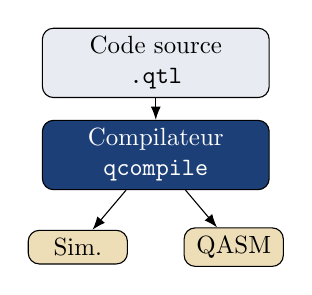
\begin{tikzpicture}[scale=0.9,every node/.style={transform shape}]
        \node[draw,rounded corners,fill=quantlblue!10,align=center,minimum width=3.2cm] (q) at (0,0) {Code source\\ \texttt{.qtl}};
        \node[draw,rounded corners,fill=quantlblue,text=white,align=center,minimum width=3.2cm] (c) at (0,-1.3) {Compilateur\\ \texttt{qcompile}};
        \node[draw,rounded corners,fill=quantlgold!30,align=center,minimum width=1.4cm] (s) at (-1.1,-2.6) {Sim.};
        \node[draw,rounded corners,fill=quantlgold!30,align=center,minimum width=1.4cm] (o) at (1.1,-2.6) {QASM};
        \draw[-{Latex}] (q) -- (c);
        \draw[-{Latex}] (c) -- (s);
        \draw[-{Latex}] (c) -- (o);
      \end{tikzpicture}
    \end{column}
  \end{columns}
\end{frame}

\begin{frame}{Objectifs du projet}
  \begin{keybox}[title=Objectif général]
    Concevoir un langage de programmation quantique compilé, complet de bout en bout : de la spécification lexicale jusqu'à la simulation numérique et l'export interopérable.
  \end{keybox}
  \vspace{4pt}
  \begin{columns}[T]
    \begin{column}{0.5\textwidth}
      \textbf{Objectifs techniques}
      \begin{itemize}
        \small
        \item Définir une grammaire formelle (EBNF/Bison) pour les circuits quantiques
        \item Construire un AST typé représentant fidèlement le programme
        \item Implémenter une analyse sémantique robuste (portées, types, usages)
        \item Générer une représentation intermédiaire (IR) linéaire et indépendante du back-end
      \end{itemize}
    \end{column}
    \begin{column}{0.5\textwidth}
      \textbf{Objectifs fonctionnels}
      \begin{itemize}
        \small
        \item Simuler l'évolution d'un état quantique par calcul matriciel sur amplitudes complexes
        \item Produire du code \textbf{OpenQASM 2.0} interopérable avec les SDK existants
        \item Offrir une interface graphique pédagogique (édition, circuit, simulation, export)
      \end{itemize}
    \end{column}
  \end{columns}
\end{frame}

% ============================================================
\section{Architecture globale du projet}
% ============================================================

\begin{frame}{Vue d'ensemble --- pipeline de compilation}
  \centering
  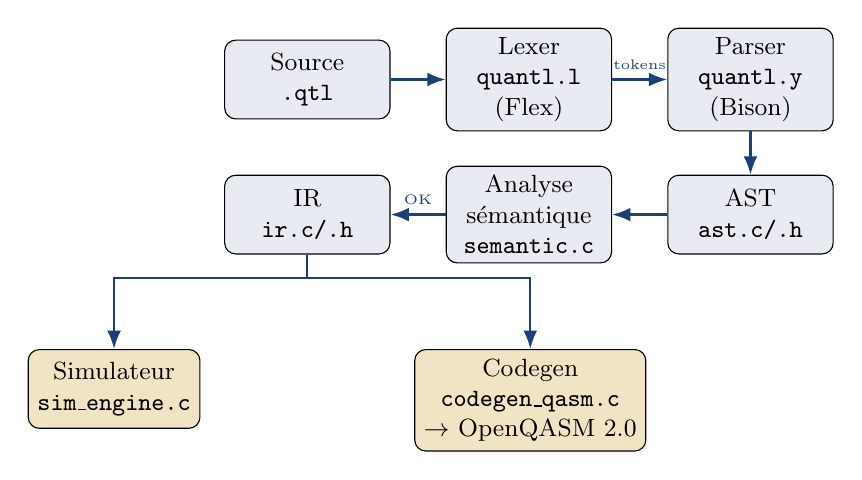
\begin{tikzpicture}[
      node distance=0.55cm and 0.7cm,
      stage/.style={draw,rounded corners,fill=quantlblue!10,minimum height=1cm,minimum width=2.1cm,align=center,font=\small},
      final/.style={draw,rounded corners,fill=quantlgold!25,minimum height=1cm,minimum width=2.1cm,align=center,font=\small},
      arr/.style={-{Latex},thick,quantlblue}
    ]
    \node[stage] (src) {Source\\ \texttt{.qtl}};
    \node[stage,right=of src] (lex) {Lexer\\ \texttt{quantl.l}\\(Flex)};
    \node[stage,right=of lex] (par) {Parser\\ \texttt{quantl.y}\\(Bison)};
    \node[stage,below=of par] (ast) {AST\\ \texttt{ast.c/.h}};
    \node[stage, left=of ast] (sem) {Analyse\\ sémantique\\ \texttt{semantic.c}};
    \node[stage,left=of sem] (ir) {IR\\ \texttt{ir.c/.h}};
    
    % Positionnement corrigé : sim et qasm en dessous de ir, l'un à gauche, l'autre à droite
    \node[final,below left=1.2cm and 0.3cm of ir] (sim) {Simulateur\\ \texttt{sim\_engine.c}};
    \node[final,below right=1.2cm and 0.3cm of ir] (qasm) {Codegen\\ \texttt{codegen\_qasm.c}\\ $\rightarrow$ OpenQASM 2.0};

    \draw[arr] (src) -- (lex);
    \draw[arr] (lex) -- node[above,font=\tiny]{tokens} (par);
    \draw[arr] (par) -- (ast);
    \draw[arr] (ast) -- (sem);
    \draw[arr] (sem) -- node[above,font=\tiny]{OK} (ir);
    
    % Flèches corrigées : partir de la face sud de ir
    \draw[arr] (ir.south) -- ++(0,-0.3) -| (sim.north);
    \draw[arr] (ir.south) -- ++(0,-0.3) -| (qasm.north);
    
  \end{tikzpicture}
  \vspace{6pt}
  {\small \\ Pipeline strictement séquentiel piloté par \texttt{main.c} (options \texttt{--source}, \texttt{--mode}, \texttt{--seed}, \texttt{--shots}).}
\end{frame}


% ============================================================
\section{Le langage QuantL}
% ============================================================

\begin{frame}{Philosophie de conception}
  \begin{itemize}
    \item Syntaxe \textbf{impérative} proche du C/OpenQASM : familière, peu de sucre syntaxique.
    \item Deux espaces de registres explicitement typés :
    \begin{itemize}
      \item \texttt{qreg} --- registre \textbf{quantique} (qubits, état en superposition)
      \item \texttt{creg} --- registre \textbf{classique} (bits résultant d'une mesure)
    \end{itemize}
    \item Toute opération référence un registre indicé : \texttt{q[0]}, \texttt{c[1]}, \dots
    \item Structures de contrôle minimales mais suffisantes pour l'enseignement : \texttt{if}, \texttt{repeat}, \texttt{barrier}.
    \item Objectif pédagogique assumé : chaque construction du langage correspond à une primitive standard de circuit quantique.
  \end{itemize}
\end{frame}

\begin{frame}[fragile]{Syntaxe --- déclarations et portes à un qubit}
  \begin{columns}[T]
    \begin{column}{0.55\textwidth}
\begin{lstlisting}[language=QuantL]
// Declarations de registres
qreg q[3];     // 3 qubits
creg c[3];     // 3 bits classiques

// Portes a un qubit (sans angle)
h q[0];        // Hadamard
x q[1];        // Pauli-X (NOT)
y q[1];        // Pauli-Y
z q[2];        // Pauli-Z
s q[0];        // Phase S
t q[0];        // Phase T (pi/4)

// Portes de rotation (avec angle)
rx q[0](pi/2);
ry q[1](1.5708);
rz q[2](pi);
\end{lstlisting}
    \end{column}
    \begin{column}{0.45\textwidth}
      \begin{keybox}[title=Table des mots-clés porte 1-qubit]
        \small
        \begin{tabular}{ll}
          \toprule
          Token & Portes \\
          \midrule
          \texttt{PORTE1Q} & h, x, y, z, s, t \\
          \texttt{PORTEROT} & rx, ry, rz \\
          \bottomrule
        \end{tabular}
      \end{keybox}
      \vspace{6pt}
      {\small Le lexer distingue les portes \emph{sans angle} des portes de \emph{rotation}, qui exigent un paramètre réel entre parenthèses (\texttt{angle : FLOTTANT | ENTIER}).}
    \end{column}
  \end{columns}
\end{frame}

\begin{frame}[fragile]{Syntaxe --- portes multi-qubits}
  \begin{columns}[T]
    \begin{column}{0.55\textwidth}
\begin{lstlisting}[language=QuantL]
// Portes a deux qubits
cx q[0], q[1];     // CNOT (controle, cible)
cz q[0], q[2];     // Controlled-Z
swap q[1], q[2];   // Echange

// Porte a trois qubits
toffoli q[0], q[1], q[2]; // CCNOT
\end{lstlisting}
    \end{column}
    \begin{column}{0.45\textwidth}
      \centering
      \begin{quantikz}[column sep=0.25cm,row sep=0.2cm]
        \lstick{$q_0$} & \ctrl{1} & \qw \\
        \lstick{$q_1$} & \targ{}  & \qw
      \end{quantikz}
      \vspace{4pt}

      \begin{quantikz}[column sep=0.25cm,row sep=0.2cm]
        \lstick{$q_0$} & \ctrl{1} & \qw \\
        \lstick{$q_1$} & \ctrl{1} & \qw \\
        \lstick{$q_2$} & \targ{}  & \qw
      \end{quantikz}
    \end{column}
  \end{columns}
\end{frame}

\begin{frame}[fragile]{Syntaxe --- mesure, contrôle conditionnel, synchronisation}
\begin{lstlisting}[language=QuantL]
// Mesure d'un qubit vers un bit classique
measure q[0] -> c[0];

// Instruction conditionnelle sur un bit classique mesure
if (c[0] == 1) x q[1];

// Barriere de synchronisation (empeche certaines optimisations)
barrier q[0], q[1], q[2];

// Repetition d'un bloc d'instructions
repeat (5) {
    h q[0];
    measure q[0] -> c[0];
}

// Affichage de diagnostics
print state;   // vecteur d'etat complet
print probs;   // distribution de probabilites + mesures
\end{lstlisting}
\end{frame}

\begin{frame}{Grammaire formelle --- extrait EBNF}
  \small
  \begin{align*}
    \textit{programme} \;&::=\; \textit{instruction}^{*} \\
    \textit{instruction} \;&::=\; \textit{decl\_qreg} \mid \textit{decl\_creg} \mid \textit{instr\_porte} \mid \textit{instr\_mesure} \\
    &\mid\; \textit{instr\_if} \mid \textit{instr\_print} \mid \textit{instr\_barrier} \mid \textit{instr\_repeat} \\
    \textit{decl\_qreg} \;&::=\; \texttt{qreg}\ \text{IDENT}\ \texttt{[}\ \text{ENTIER}\ \texttt{]}\ \texttt{;} \\
    \textit{instr\_porte} \;&::=\; \text{PORTE1Q}\ \text{IDENT[ENTIER]}\ (\texttt{(}\textit{angle}\texttt{)})^{?}\ \texttt{;} \\
    &\mid\; \text{PORTE2Q}\ \text{IDENT[ENTIER]}\texttt{,}\ \text{IDENT[ENTIER]}\ \texttt{;} \\
    &\mid\; \texttt{toffoli}\ \text{IDENT[ENTIER]}\texttt{,}\ \text{IDENT[ENTIER]}\texttt{,}\ \text{IDENT[ENTIER]}\ \texttt{;} \\
    \textit{instr\_if} \;&::=\; \texttt{if (}\text{IDENT[ENTIER]}\ \texttt{==}\ \text{ENTIER}\texttt{)}\ \textit{instruction} \\
    \textit{instr\_repeat} \;&::=\; \texttt{repeat (}\text{ENTIER}\texttt{) \{}\ \textit{instruction}^{*}\ \texttt{\}} \\
    \textit{angle} \;&::=\; \text{FLOTTANT} \mid \text{ENTIER}
  \end{align*}
  \begin{warnbox}[title=Remarque]
    La grammaire est implémentée directement en \textbf{Bison} (\texttt{quantl.y}) avec \texttt{\%define parse.error verbose} pour des messages d'erreur syntaxique explicites, et gérée sans conflits shift/reduce résiduels (\texttt{-v} génère \texttt{quantl.output}).
  \end{warnbox}
\end{frame}

% ============================================================
\section{Analyse lexicale et syntaxique}
% ============================================================

\begin{frame}[fragile]{Analyseur lexical (Flex) --- \texttt{quantl.l}}
  \begin{columns}[T]
    \begin{column}{0.55\textwidth}
\begin{lstlisting}[style=cstyle]
"qreg"  { return QREG; }
"creg"  { return CREG; }
"h"|"x"|"y"|"z"|"s"|"t"
        { yylval.str = strdup(yytext);
          return PORTE1Q; }
"rx"|"ry"|"rz"
        { yylval.str = strdup(yytext);
          return PORTEROT; }
"cx"|"cz"|"swap"
        { yylval.str = strdup(yytext);
          return PORTE2Q; }
"pi"    { yylval.dval = 3.14159265358979;
          return FLOTTANT; }
[a-zA-Z_][a-zA-Z0-9_]*
        { yylval.str = strdup(yytext);
          return IDENT; }
\end{lstlisting}
    \end{column}
    \begin{column}{0.45\textwidth}
      \textbf{Caractéristiques}
      \begin{itemize}
        \small
        \item Reconnaissance des mots-clés \emph{avant} la règle générique \texttt{IDENT} (priorité à la règle la plus longue/la plus spécifique de Flex)
        \item Gestion du comptage de lignes (\texttt{ligne\_courante}) pour les diagnostics d'erreur
        \item Ignore les commentaires \texttt{//...} et les espaces/tabulations
        \item Rejette proprement les caractères invalides avec message d'erreur explicite (protection contre BOM/Unicode invisibles)
        \item Constante \texttt{pi} injectée directement comme littéral flottant au niveau lexical
      \end{itemize}
    \end{column}
  \end{columns}
\end{frame}

\begin{frame}[fragile]{Analyseur syntaxique (Bison) --- règle \texttt{instr\_if}}
\begin{lstlisting}[style=cstyle]
instr_if:
    IF '(' IDENT '[' ENTIER ']' EGALEGAL ENTIER ')'
    instruction {
        $$ = ast_if($3, $5, $8, $10, ligne_courante);
    }
    ;
\end{lstlisting}
  \begin{itemize}
    \item La règle \texttt{instr\_if} est \textbf{récursive à droite} : le corps du \texttt{if} est lui-même une \textit{instruction} quelconque (porte, mesure, print, etc.), pas un bloc obligatoire.
    \item Les valeurs sémantiques (\texttt{\$3}, \texttt{\$5}, \dots) sont combinées via \texttt{ast\_if(...)} pour construire un nœud \texttt{N\_IF} homogène.
    \item L'union Bison \texttt{\%union} porte quatre types de valeurs : \texttt{ival}, \texttt{dval}, \texttt{str}, \texttt{noeud} --- reflet direct des types de tokens (\texttt{ENTIER}, \texttt{FLOTTANT}, \texttt{IDENT}, non-terminaux).
    \item La règle \texttt{liste\_ref\_qubits} (pour \texttt{barrier}) illustre une construction incrémentale par \texttt{realloc} d'un tableau de \texttt{Reference}.
  \end{itemize}
\end{frame}

% ============================================================
\section{Arbre syntaxique abstrait (AST)}
% ============================================================

\begin{frame}[fragile]{Structure de données de l'AST}
  \begin{columns}[T]
    \begin{column}{0.52\textwidth}
\begin{lstlisting}[style=cstyle]
typedef struct NoeudAST {
    TypeNoeud type;
    int ligne;
    struct NoeudAST* suivant;
    union {
        struct { char* nom_registre;
                 int taille;
                 TypeRegistre type_reg; } decl;
        struct { char* nom_porte;
                 char* nom_reg;
                 int indice_qubit;
                 double angle;
                 bool a_angle; } porte_1q;
        struct { ... } porte_2q;
        struct { ... } porte_toffoli;
        struct { ... } mesure;
        struct { ... } if_instr;
        struct { ... } print_instr;
        struct { ... } barrier;
        struct { ... } repeat;
    };
} NoeudAST;
\end{lstlisting}
    \end{column}
    \begin{column}{0.48\textwidth}
      \textbf{Points clés de conception}
      \begin{itemize}
        \small
        \item Un \textbf{unique type de nœud} (\texttt{NoeudAST}) avec une \texttt{union} discriminée par le champ \texttt{type} (\texttt{TypeNoeud})
        \item Chaînage \texttt{suivant} $\to$ liste simplement chaînée d'instructions (pas d'arbre n-aire classique)
        \item Chaque instruction porte son \textbf{numéro de ligne} pour la traçabilité des erreurs
        \item Les instructions composées (\texttt{if}, \texttt{repeat}) embarquent un pointeur vers un sous-AST (\texttt{instruction} / \texttt{bloc})
        \item Fonctions de construction dédiées : \texttt{ast\_decl\_registre}, \texttt{ast\_porte\_1q}, \texttt{ast\_if}, etc.
      \end{itemize}
    \end{column}
  \end{columns}
\end{frame}

\begin{frame}{AST --- exemple : état de Bell}
  \centering
  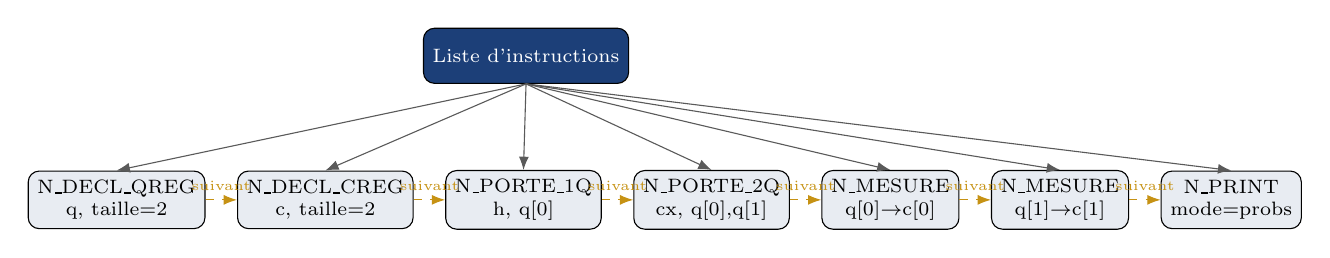
\begin{tikzpicture}[
      node distance=0.5cm and 0.4cm,
      nd/.style={draw,rounded corners,fill=quantlblue!10,align=center,font=\scriptsize,minimum height=0.7cm},
      arr/.style={-{Latex},quantlgray}
    ]
    \node[nd,fill=quantlblue,text=white] (root) {Liste d'instructions};
    \node[nd,below=1.1cm of root,xshift=-5.2cm] (n1) {N\_DECL\_QREG\\ q, taille=2};
    \node[nd,right=of n1] (n2) {N\_DECL\_CREG\\ c, taille=2};
    \node[nd,right=of n2] (n3) {N\_PORTE\_1Q\\ h, q[0]};
    \node[nd,right=of n3] (n4) {N\_PORTE\_2Q\\ cx, q[0],q[1]};
    \node[nd,right=of n4] (n5) {N\_MESURE\\ q[0]$\to$c[0]};
    \node[nd,right=of n5] (n6) {N\_MESURE\\ q[1]$\to$c[1]};
    \node[nd,right=of n6] (n7) {N\_PRINT\\ mode=probs};

    \foreach \n in {n1,n2,n3,n4,n5,n6,n7}
      \draw[arr] (root.south) -- (\n.north);
    \draw[-{Latex},dashed,quantlgold] (n1.east) -- (n2.west) node[midway,above,font=\tiny]{suivant};
    \draw[-{Latex},dashed,quantlgold] (n2.east) -- (n3.west) node[midway,above,font=\tiny]{suivant};
    \draw[-{Latex},dashed,quantlgold] (n3.east) -- (n4.west) node[midway,above,font=\tiny]{suivant};
    \draw[-{Latex},dashed,quantlgold] (n4.east) -- (n5.west) node[midway,above,font=\tiny]{suivant};
    \draw[-{Latex},dashed,quantlgold] (n5.east) -- (n6.west) node[midway,above,font=\tiny]{suivant};
    \draw[-{Latex},dashed,quantlgold] (n6.east) -- (n7.west) node[midway,above,font=\tiny]{suivant};
  \end{tikzpicture}
  \vspace{6pt}

  {\small La liste chaînée (\alert{flèches en pointillé} = champ \texttt{suivant}) reflète l'ordre séquentiel du programme source, tandis que chaque nœud encapsule ses attributs propres via l'union.}
\end{frame}

% ============================================================
\section{Analyse sémantique}
% ============================================================

\begin{frame}{Rôle de l'analyse sémantique (\texttt{semantic.c})}
  \begin{itemize}
    \item Parcourt l'AST une seconde fois pour vérifier des propriétés que la grammaire seule ne peut exprimer.
    \item Maintient une \textbf{table des symboles} chaînée (\texttt{Symbole}) : nom, type (\texttt{QUANTIQUE}/\texttt{CLASSIQUE}), taille, ligne de déclaration, et pour les registres classiques un tableau \texttt{bool* mesure} (bit déjà mesuré ou non).
    \item Comptabilise le nombre total de qubits déclarés (\texttt{nb\_qubits\_total}) avec avertissement au-delà de \texttt{MAX\_QUBITS = 20} (limite dictée par la taille $2^n$ de l'espace d'état simulé).
  \end{itemize}
  \begin{keybox}[title=Fonctions clés]
    \small
    \texttt{trouver\_symbole}, \texttt{ajouter\_symbole}, \texttt{verifier\_reference} (bornes d'indice), \texttt{marquer\_mesure} / \texttt{bit\_est\_mesure}, \texttt{analyser\_noeud} (dispatch par \texttt{TypeNoeud})
  \end{keybox}
\end{frame}

\begin{frame}{Règles de vérification statique}
  \small
  \begin{tabular}{@{}p{6.3cm}p{5.3cm}@{}}
    \toprule
    \textbf{Vérification} & \textbf{Sévérité} \\
    \midrule
    Registre redéclaré sous le même nom & Erreur \\
    Registre inconnu / indice hors bornes & Erreur \\
    Porte quantique appliquée à un registre classique & Erreur \\
    Angle manquant pour une porte de rotation & Erreur \\
    Angle fourni pour une porte sans paramètre & Avertissement \\
    Contrôle et cible identiques (\texttt{cx}, \texttt{cz}, Toffoli) & Erreur \\
    Mesure vers un registre non classique / depuis un registre non quantique & Erreur \\
    Condition \texttt{if} portant sur un registre quantique & Erreur \\
    Bit classique testé dans un \texttt{if} sans avoir été mesuré au préalable & Avertissement \\
    \bottomrule
  \end{tabular}
  \vspace{6pt}
  \begin{warnbox}[title=Exemple de diagnostic]
    \ttfamily\scriptsize Erreur sémantique (ligne 7) : Porte quantique sur registre classique 'c'.
  \end{warnbox}
\end{frame}

% ============================================================
\section{Représentation intermédiaire (IR)}
% ============================================================

\begin{frame}[fragile]{Structure de l'IR --- \texttt{ir.h}}
\begin{lstlisting}[style=cstyle]
typedef enum {
    OP_H, OP_X, OP_Y, OP_Z, OP_S, OP_T,
    OP_RX, OP_RY, OP_RZ,
    OP_CX, OP_CZ, OP_SWAP, OP_TOFFOLI,
    OP_MEASURE, OP_IF_DEBUT, OP_IF_FIN,
    OP_BARRIER, OP_PRINT_STATE, OP_PRINT_PROBS
} OpCode;

typedef struct InstructionIR {
    OpCode op;
    int qubits[3];       int nb_qubits;
    int bit_classique;   double angle;
    int condition_bit;   int condition_val;
    int ligne_source;    int registre_id;
    struct InstructionIR *suivant;
} InstructionIR;
\end{lstlisting}
  \begin{itemize}
    \small
    \item L'IR est une \textbf{liste linéaire} d'instructions à plat : les qubits multi-registres sont ramenés à des \textbf{indices globaux} via une table \texttt{RegistreMapping} (nom $\to$ qubit de départ, taille).
    \item Les blocs \texttt{if} sont \emph{aplatis} en une paire de marqueurs \texttt{OP\_IF\_DEBUT} / \texttt{OP\_IF\_FIN} encadrant les instructions conditionnelles --- indépendant du back-end consommateur (simulateur ou QASM).
  \end{itemize}
\end{frame}

\begin{frame}{De l'AST à l'IR --- indépendance des back-ends}
  \centering
  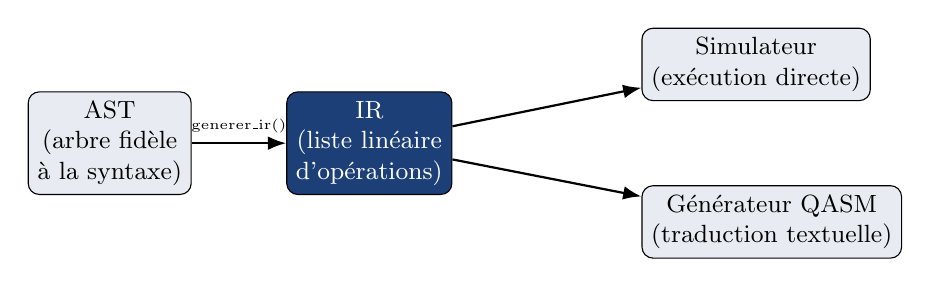
\begin{tikzpicture}[
      node distance=0.6cm and 1.2cm,
      nd/.style={draw,rounded corners,fill=quantlblue!10,align=center,font=\small,minimum height=0.9cm}
    ]
    \node[nd] (ast) {AST\\(arbre fidèle\\à la syntaxe)};
    \node[nd,right=of ast,fill=quantlblue,text=white] (ir) {IR\\(liste linéaire\\d'opérations)};
    \node[nd,right=2.4cm of ir,yshift=1cm] (sim) {Simulateur\\(exécution directe)};
    \node[nd,right=2.4cm of ir,yshift=-1cm] (qasm) {Générateur QASM\\(traduction textuelle)};
    \draw[-{Latex},thick] (ast) -- node[above,font=\tiny]{generer\_ir()} (ir);
    \draw[-{Latex},thick] (ir) -- (sim);
    \draw[-{Latex},thick] (ir) -- (qasm);
  \end{tikzpicture}
  \vspace{8pt}

  \begin{itemize}
    \item L'IR découple la \emph{sémantique du langage} de son \emph{exécution} : un même flux d'\texttt{InstructionIR} alimente indifféremment le simulateur ou le générateur de code.
    \item Ce découplage facilite l'ajout futur d'autres back-ends (ex. transpilation vers un SDK tiers) sans toucher au front-end (lexer/parser/AST).
  \end{itemize}
\end{frame}

% ============================================================
\section{Moteur de simulation quantique}
% ============================================================

\begin{frame}{Modèle mathématique --- vecteur d'état}
  \begin{itemize}
    \item Un registre de $n$ qubits est représenté par un vecteur complexe de dimension $2^n$ :
    \[
      \ket{\psi} = \sum_{i=0}^{2^n-1} \alpha_i \ket{i}, \qquad \alpha_i \in \mathbb{C}, \qquad \sum_i |\alpha_i|^2 = 1
    \]
    \item Implémentation : \texttt{double complex* etat} de taille \texttt{1 << nb\_qubits}, initialisé à $\ket{0\ldots0}$ (\texttt{etat[0] = 1.0}).
    \item Une porte à 1 qubit sur le qubit $k$ agit par \textbf{paires d'indices} $(i, i \oplus 2^k)$ : c'est le c\oe ur de \texttt{sim\_appliquer\_porte\_1q}, qui applique une matrice $2\times2$ à chaque paire sans reconstruire l'état complet.
  \end{itemize}
  \begin{keybox}[title=Complexité]
    Chaque porte 1-qubit coûte $O(2^n)$ ; la limite \texttt{MAX\_QUBITS=20} borne la mémoire à $2^{20}$ amplitudes complexes ($\approx$ 16 Mo en \texttt{double complex}).
  \end{keybox}
\end{frame}

\begin{frame}{Portes à un qubit --- matrices implémentées}
  \small
  \begin{columns}[T]
    \begin{column}{0.5\textwidth}
      \[
        H = \tfrac{1}{\sqrt2}\begin{pmatrix}1&1\\1&-1\end{pmatrix} \quad
        X = \begin{pmatrix}0&1\\1&0\end{pmatrix} \quad
        Y = \begin{pmatrix}0&-i\\i&0\end{pmatrix}
      \]
      \[
        Z = \begin{pmatrix}1&0\\0&-1\end{pmatrix} \quad
        S = \begin{pmatrix}1&0\\0&i\end{pmatrix} \quad
        T = \begin{pmatrix}1&0\\0&e^{i\pi/4}\end{pmatrix}
      \]
    \end{column}
    \begin{column}{0.5\textwidth}
      \[
        R_x(\theta) = \begin{pmatrix}\cos\frac{\theta}{2} & -i\sin\frac{\theta}{2}\\-i\sin\frac{\theta}{2} & \cos\frac{\theta}{2}\end{pmatrix}
      \]
      \[
        R_y(\theta) = \begin{pmatrix}\cos\frac{\theta}{2} & -\sin\frac{\theta}{2}\\ \sin\frac{\theta}{2} & \cos\frac{\theta}{2}\end{pmatrix}
      \]
      \[
        R_z(\theta) = \begin{pmatrix}e^{-i\theta/2} & 0\\0 & e^{i\theta/2}\end{pmatrix}
      \]
    \end{column}
  \end{columns}
  \vspace{4pt}
  {\footnotesize Chaque matrice est construite localement dans \texttt{sim\_appliquer\_ir} (dispatch sur \texttt{OpCode}) puis déléguée à la fonction générique \texttt{sim\_appliquer\_porte\_1q}.}
\end{frame}

\begin{frame}{Portes multi-qubits --- implémentation par permutation/phase}
  \begin{itemize}
    \item \textbf{CX (CNOT)} : pour tout indice $i$ avec le bit de contrôle à 1, échange les amplitudes $i$ et $i \oplus 2^{\text{cible}}$ (\texttt{sim\_appliquer\_cx}).
    \item \textbf{CZ} : applique une phase $-1$ lorsque les deux bits (contrôle \emph{et} cible) valent 1 --- aucune permutation nécessaire (\texttt{sim\_appliquer\_cz}).
    \item \textbf{SWAP} : échange les amplitudes correspondant à l'inversion des bits $q_1$ et $q_2$ (\texttt{sim\_appliquer\_swap}).
    \item \textbf{Toffoli (CCNOT)} : généralisation du CNOT à deux contrôles ; échange $i \leftrightarrow i \oplus 2^{\text{cible}}$ si les deux bits de contrôle valent 1 (\texttt{sim\_appliquer\_toffoli}).
  \end{itemize}
  \begin{keybox}[title=Observation]
    Toutes ces portes sont \textbf{unitaires par construction} car implémentées comme des permutations d'amplitudes (ou des changements de phase de module 1), garantissant la conservation de la norme sans vérification explicite supplémentaire.
  \end{keybox}
\end{frame}

\begin{frame}{Mesure quantique --- probabilités et effondrement}
  \begin{enumerate}
    \item Calcul de $p_0 = \sum_{i : \text{bit}_k(i)=0} |\alpha_i|^2$ (probabilité d'obtenir 0 sur le qubit $k$).
    \item Tirage d'un nombre pseudo-aléatoire $r \sim \mathcal{U}(0,1)$ via \texttt{rand()} (graine \texttt{srand(seed)} pour la reproductibilité, ou \texttt{time(NULL)} sinon).
    \item Résultat $= 1$ si $r > p_0$, sinon $0$ ; le bit classique correspondant est mis à jour.
    \item \textbf{Projection} : toutes les amplitudes incompatibles avec le résultat sont mises à zéro.
    \item \textbf{Renormalisation} : division par $\sqrt{\text{norme restante}}$ pour restaurer $\sum|\alpha_i|^2 = 1$.
  \end{enumerate}
  \begin{warnbox}[title=Point d'attention identifié]
    Le test \texttt{r > p0} pour choisir le résultat 1 est une convention arbitraire mais cohérente ; la reproductibilité totale d'une exécution dépend uniquement de la graine passée en \texttt{--seed}.
  \end{warnbox}
\end{frame}

\begin{frame}[fragile]{Structures de contrôle dans l'IR --- exemple \texttt{if}}
\begin{lstlisting}[style=cstyle]
case OP_IF_DEBUT: {
    int val = sim->bits_classiques[courant->condition_bit];
    if (val == courant->condition_val) {
        courant = courant->suivant;
        while (courant && courant->op != OP_IF_FIN) {
            sim_appliquer_ir(sim, courant);
            courant = courant->suivant;
        }
    } else {
        while (courant && courant->op != OP_IF_FIN) {
            courant = courant->suivant;
        }
    }
    break;
}
\end{lstlisting}
  {\small Le simulateur interprète directement la paire \texttt{OP\_IF\_DEBUT}/\texttt{OP\_IF\_FIN} comme un \emph{saut conditionnel} sur la liste chaînée d'IR --- sans backpatching ni structure arborescente, contrairement à l'AST.}
\end{frame}

% ============================================================
\section{Génération de code OpenQASM 2.0}
% ============================================================

\begin{frame}[fragile]{Export vers OpenQASM 2.0 (\texttt{codegen\_qasm.c})}
  \begin{columns}[T]
    \begin{column}{0.5\textwidth}
      \textbf{Principe}
      \begin{itemize}
        \small
        \item Un unique parcours de l'IR détermine \texttt{nb\_qubits} et \texttt{nb\_bits} par balayage des champs \texttt{qubits[]} / \texttt{bit\_classique}.
        \item En-tête standard généré automatiquement :
      \end{itemize}
\begin{lstlisting}[basicstyle=\ttfamily\tiny]
OPENQASM 2.0;
include "qelib1.inc";
qreg q[N]; creg c[M];
\end{lstlisting}
      \begin{itemize}
        \small
        \item Traduction directe \texttt{OpCode} $\to$ instruction QASM (\texttt{h}, \texttt{cx}, \texttt{rz(theta)}, \texttt{measure ... -> ...}, \texttt{if (c==v) \{ ... \}}, \texttt{barrier}, \texttt{ccx} pour Toffoli).
        \item Les \texttt{print state}/\texttt{print probs} (propres à la simulation) sont convertis en \textbf{commentaires} QASM.
      \end{itemize}
    \end{column}
    \begin{column}{0.5\textwidth}
\begin{lstlisting}[basicstyle=\ttfamily\tiny,frame=single]
OPENQASM 2.0;
include "qelib1.inc";

qreg q[2];
creg c[2];

h q[0];
cx q[0], q[1];
measure q[0] -> c[0];
measure q[1] -> c[1];
// print probs (simulation uniquement)
\end{lstlisting}
      {\footnotesize Sortie réelle pour le programme \texttt{bell.qtl} --- directement importable dans Qiskit, IBM Quantum Experience ou tout outil compatible OpenQASM 2.0.}
    \end{column}
  \end{columns}
\end{frame}

% ============================================================
\section{Étude de cas : trois circuits de référence}
% ============================================================

\begin{frame}[fragile]{Cas d'étude 1 --- État de Bell (intrication à 2 qubits)}
  \begin{columns}[T]
    \begin{column}{0.42\textwidth}
\begin{lstlisting}[language=QuantL]
qreg q[2];
creg c[2];

h q[0];
cx q[0], q[1];

measure q[0] -> c[0];
measure q[1] -> c[1];

print probs;
\end{lstlisting}
    \end{column}
    \begin{column}{0.58\textwidth}
      \centering
      \begin{quantikz}[column sep=0.3cm]
        \lstick{$q_0 : \ket{0}$} & \gate{H} & \ctrl{1} & \meter{} & \qw \\
        \lstick{$q_1 : \ket{0}$} & \qw      & \targ{}  & \meter{} & \qw
      \end{quantikz}

      \vspace{6pt}
      \[
        \ket{\psi} = \tfrac{1}{\sqrt2}\big(\ket{00} + \ket{11}\big)
      \]
      {\small Résultats attendus (\texttt{print probs}) : $P(00)=P(11)=0.5$, $P(01)=P(10)=0$ --- corrélation parfaite entre \texttt{c[0]} et \texttt{c[1]}.}
    \end{column}
  \end{columns}
\end{frame}

\begin{frame}[fragile]{Cas d'étude 2 --- État GHZ (intrication à 3 qubits)}
  \begin{columns}[T]
    \begin{column}{0.42\textwidth}
\begin{lstlisting}[language=QuantL]
qreg q[3];
creg c[3];

h q[0];
cx q[0], q[1];
cx q[1], q[2];

barrier q[0], q[1], q[2];

measure q[0] -> c[0];
measure q[1] -> c[1];
measure q[2] -> c[2];

print probs;
\end{lstlisting}
    \end{column}
    \begin{column}{0.58\textwidth}
      \centering
      \begin{quantikz}[column sep=0.25cm,row sep=0.15cm]
        \lstick{$q_0$} & \gate{H} & \ctrl{1} & \qw      & \qw      & \meter{} & \qw \\
        \lstick{$q_1$} & \qw      & \targ{}  & \ctrl{1} & \qw      & \meter{} & \qw \\
        \lstick{$q_2$} & \qw      & \qw      & \targ{}  & \qw      & \meter{} & \qw
      \end{quantikz}
      \vspace{6pt}
      \[
        \ket{\psi} = \tfrac{1}{\sqrt2}\big(\ket{000} + \ket{111}\big)
      \]
      {\small La \texttt{barrier} illustre la synchronisation explicite avant mesure --- sans effet sur l'état simulé mais préservée dans l'export QASM.}
    \end{column}
  \end{columns}
\end{frame}

\begin{frame}[fragile]{Cas d'étude 3 --- Algorithme de Deutsch}
  \begin{columns}[T]
    \begin{column}{0.42\textwidth}
\begin{lstlisting}[language=QuantL]
qreg q[2];
creg c[1];

x q[1];
h q[0];
h q[1];

cx q[0], q[1];

h q[0];
measure q[0] -> c[0];

if (c[0] == 0) print state;
if (c[0] == 1) print state;
\end{lstlisting}
    \end{column}
    \begin{column}{0.58\textwidth}
      \centering
      \begin{quantikz}[column sep=0.22cm,row sep=0.15cm]
        \lstick{$q_0:\ket{0}$} & \gate{H} & \ctrl{1} & \gate{H} & \meter{} & \qw \\
        \lstick{$q_1:\ket{1}$} & \gate{H} & \targ{}  & \qw      & \qw      & \qw
      \end{quantikz}
      \vspace{6pt}
      \begin{itemize}
        \small
        \item Illustre l'oracle $U_f$ implémenté ici via \texttt{cx} (fonction équilibrée $f(x)=x$).
        \item Démontre l'usage du couple \texttt{if}/\texttt{print} pour un diagnostic conditionnel post-mesure --- test direct des règles sémantiques sur les registres classiques mesurés.
      \end{itemize}
    \end{column}
  \end{columns}
\end{frame}

% ============================================================
\section{Interface graphique (PyQt6)}
% ============================================================

\begin{frame}{Architecture MVC de la GUI}
  \centering
  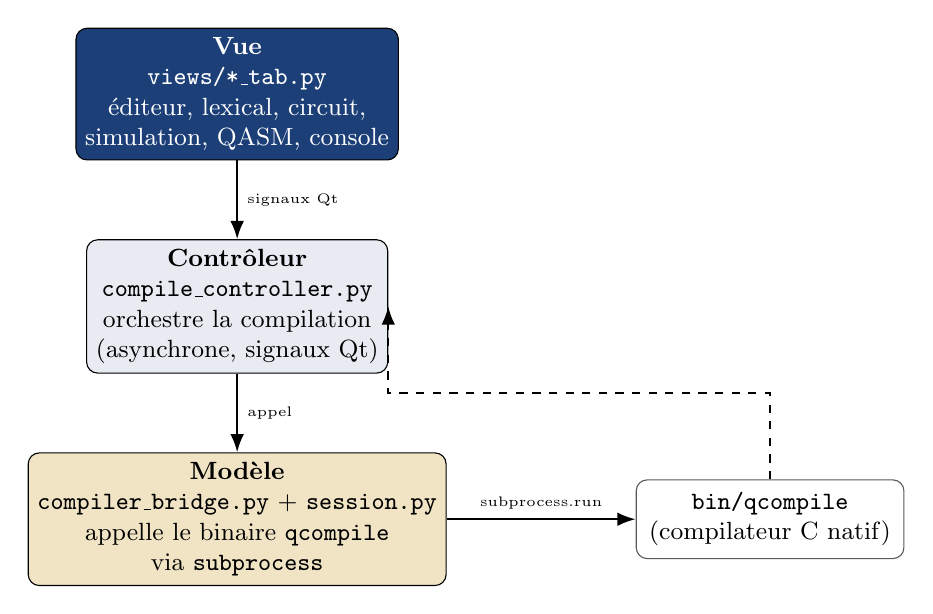
\begin{tikzpicture}[
      node distance=1.0cm and 1.4cm,
      nd/.style={draw,rounded corners,fill=quantlblue!10,align=center,font=\small,minimum width=3.4cm,minimum height=1cm}
    ]
    \node[nd,fill=quantlblue,text=white] (view) {\textbf{Vue} \\ \texttt{views/*\_tab.py}\\ éditeur, lexical, circuit,\\ simulation, QASM, console};
    \node[nd,below=of view] (ctrl) {\textbf{Contrôleur} \\ \texttt{compile\_controller.py}\\ orchestre la compilation\\ (asynchrone, signaux Qt)};
    \node[nd,below=of ctrl,fill=quantlgold!25] (model) {\textbf{Modèle} \\ \texttt{compiler\_bridge.py} + \texttt{session.py}\\ appelle le binaire \texttt{qcompile}\\ via \texttt{subprocess}};
    \node[nd,right=2.4cm of model,fill=white,draw=quantlgray] (bin) {\texttt{bin/qcompile}\\ (compilateur C natif)};

    \draw[-{Latex},thick] (view) -- node[right,font=\tiny]{signaux Qt} (ctrl);
    \draw[-{Latex},thick] (ctrl) -- node[right,font=\tiny]{appel} (model);
    \draw[-{Latex},thick] (model) -- node[above,font=\tiny]{subprocess.run} (bin);
    \draw[-{Latex},thick,dashed] (bin) -- ++(0,1.6) -| (ctrl.east);
  \end{tikzpicture}
  \vspace{6pt}
  {\small Le \texttt{CompilerBridge} localise dynamiquement l'exécutable \texttt{qcompile} (plusieurs chemins candidats testés), l'invoque avec un fichier temporaire \texttt{.qtl}, puis parse \texttt{stdout}/\texttt{stderr} pour reconstituer un résultat structuré.}
\end{frame}

\begin{frame}{Organisation des onglets de résultats}
  \begin{columns}[T]
    \begin{column}{0.5\textwidth}
      \begin{itemize}
        \item \textbf{Éditeur} --- panneau permanent (splitter gauche), coloration syntaxique QuantL
        \item \textbf{Lexical / Syntaxique} --- visualisation des tokens et de l'AST
        \item \textbf{Circuit} --- représentation graphique du circuit quantique
        \item \textbf{Simulation} --- vecteur d'état, probabilités, résultats de mesure
      \end{itemize}
    \end{column}
    \begin{column}{0.5\textwidth}
      \begin{itemize}
        \item \textbf{Export QASM} --- code OpenQASM 2.0 généré, copiable/exportable
        \item \textbf{Console} --- sortie brute du compilateur (diagnostics, erreurs)
        \item Thèmes \textbf{clair/sombre} interchangeables (\texttt{light.qss} / \texttt{dark.qss})
        \item Exemples préchargés : État de Bell, GHZ, Deutsch (menu \texttt{EXAMPLES})
      \end{itemize}
    \end{column}
  \end{columns}
  \vspace{8pt}
  \begin{keybox}[title=Ergonomie]
    Contrairement à une interface purement à onglets, l'éditeur reste \textbf{toujours visible} à gauche (via un \texttt{QSplitter}) : l'utilisateur ne perd jamais le contexte du code source en consultant les résultats.
  \end{keybox}
\end{frame}

% ============================================================
\section{Compilation, tests et validation}
% ============================================================

\begin{frame}[fragile]{Chaîne de build (Makefile)}
\begin{lstlisting}[basicstyle=\ttfamily\scriptsize]
quantl.y --(bison -d -v)--> quantl.tab.c / quantl.tab.h
quantl.l --(flex)---------> quantl.yy.c
*.c       --(gcc -std=c11 -Wall -Wextra -O2)--> build/*.o
build/*.o --(gcc, -lm)--------------------------> bin/qcompile
\end{lstlisting}
  \begin{itemize}
    \small
    \item Compilation stricte : \texttt{-Wall -Wextra -std=c11}, liaison avec \texttt{libm} (fonctions trigonométriques/complexes).
    \item Cible \texttt{make test} exécute automatiquement les trois programmes de référence (\texttt{bell.qtl}, \texttt{ghz.qtl}, \texttt{deutsch.qtl}) avec une graine fixe (\texttt{--seed 12345}) pour des résultats reproductibles.
    \item Cibles \texttt{clean} / \texttt{distclean} pour la suppression des artefacts générés (\texttt{.o}, binaire, fichiers Bison/Flex intermédiaires, \texttt{.qasm}).
  \end{itemize}
\end{frame}

\begin{frame}{Suite de tests}
  \begin{columns}[T]
    \begin{column}{0.5\textwidth}
      \textbf{Tests fonctionnels (\texttt{tests/})}
      \begin{itemize}
        \small
        \item \texttt{bell.qtl}, \texttt{ghz.qtl}, \texttt{deutsch.qtl} --- circuits de référence complets
        \item \texttt{simple.qtl}, \texttt{bell\_debug.qtl} --- cas minimaux de débogage
      \end{itemize}
    \end{column}
    \begin{column}{0.5\textwidth}
      \textbf{Tests structurés par phase}
      \begin{itemize}
        \small
        \item \texttt{lexical\_tests/} --- validation du tokenizer
        \item \texttt{syntax\_tests/} --- validation de la grammaire
        \item \texttt{semantic\_tests/} --- validation des règles statiques
      \end{itemize}
    \end{column}
  \end{columns}
  \vspace{10pt}
  \begin{keybox}[title=Reproductibilité]
    L'option \texttt{--seed N} garantit qu'une même exécution produit toujours les mêmes résultats de mesure, condition nécessaire pour des tests automatisés déterministes sur un phénomène par nature probabiliste.
  \end{keybox}
\end{frame}

% ============================================================
\section{Bilan, limites et perspectives}
% ============================================================

\begin{frame}{Bilan du projet}
  \begin{keybox}[title=Ce qui est fonctionnel de bout en bout]
    \small
    Lexer $\to$ Parser $\to$ AST $\to$ Analyse sémantique $\to$ IR $\to$ \{Simulateur, Export QASM 2.0\}, avec interface graphique complète appelant le compilateur natif.
  \end{keybox}
  \vspace{4pt}
  \begin{itemize}
    \item Couverture des primitives essentielles du calcul quantique par circuits : portes 1/2/3-qubits, mesure, contrôle conditionnel classique, synchronisation, répétition.
    \item Simulateur numériquement correct par construction (portes unitaires implémentées comme permutations/phases sur le vecteur d'état).
    \item Interopérabilité assurée via l'export OpenQASM 2.0, standard reconnu de l'écosystème (Qiskit, IBM Quantum).
  \end{itemize}
\end{frame}

\begin{frame}{Limites actuelles}
  \begin{itemize}
    \item \textbf{Simulation idéale uniquement} : aucun modèle de bruit (dépolarisation, relaxation $T_1/T_2$, portes bruitées) --- le simulateur suppose un matériel parfait.
    \item \textbf{Passage à l'échelle} : complexité mémoire en $O(2^n)$, limite pragmatique fixée à 20 qubits (16 Mo d'amplitudes complexes).
    \item \textbf{Pas d'optimisation de circuit} : aucune fusion/réécriture de portes avant simulation ou export (contrairement aux transpileurs de SDK matures).
    \item \texttt{repeat} génère une ré-exécution complète du bloc à chaque simulation, sans réutilisation d'état entre itérations autre que via les registres classiques.
    \item Le fichier \texttt{json\_writer.c/.h} est présent mais vide --- fonctionnalité d'export JSON planifiée mais non implémentée.
  \end{itemize}
\end{frame}

\begin{frame}{Perspectives d'évolution}
  \begin{columns}[T]
    \begin{column}{0.5\textwidth}
      \textbf{Extensions du langage}
      \begin{itemize}
        \small
        \item Fonctions/sous-circuits réutilisables (modularité)
        \item Boucles paramétrées par variable (au-delà de \texttt{repeat(N)} constant)
        \item Types de données classiques plus riches (entiers signés, tableaux)
      \end{itemize}
      \textbf{Modèle physique}
      \begin{itemize}
        \small
        \item Modélisation du bruit et de la décohérence
        \item Bascule vers un back-end \textbf{Qiskit} réel pour exécution sur matériel/simulateurs cloud
      \end{itemize}
    \end{column}
    \begin{column}{0.5\textwidth}
      \textbf{Outillage}
      \begin{itemize}
        \small
        \item Optimiseur de circuits (fusion de portes, réduction de profondeur)
        \item Export JSON structuré (finaliser \texttt{json\_writer})
        \item Visualisation graphique interactive du circuit dans l'onglet \emph{Circuit}
        \item Tests automatisés end-to-end intégrés (CI)
      \end{itemize}
    \end{column}
  \end{columns}
\end{frame}

\begin{frame}{Conclusion}
  \begin{keybox}[title=Synthèse]
    QuantL démontre qu'il est possible de bâtir, avec des outils de compilation classiques (\textbf{Flex}, \textbf{Bison}, \textbf{C}), un langage dédié à la programmation de circuits quantiques, complet depuis l'analyse lexicale jusqu'à la simulation numérique et l'interopérabilité via OpenQASM, le tout encapsulé dans une interface graphique accessible (\textbf{PyQt6}).
  \end{keybox}
  \vspace{10pt}
  \centering
  \Large \textcolor{quantlblue}{\textbf{Merci de votre attention}}

  \vspace{6pt}
  \normalsize Questions \& discussion
\end{frame}

\end{document}
